\section{Εργαλεία Και Τεχνικές}
\subsection{Πλαίσιο Λογισμικού - PHP}
Για την υλοποίηση του REST API χρησιμοποιήθηκε το framework\footnotemark\footnotetext{Software framework, a reusable set of libraries or classes for a software system} \textbf{Lumen-Laravel} \cite{lumen-laravel} που ενδείκνυται για το σκοπό αυτό. Ωστόσο τα προαπαιτούμενα για την χρήση του framework είναι:  

\begin{itemize}
\item PHP >= 5.6.4
\item OpenSSL PHP Extension
\item PDO PHP Extension
\item Mbstring PHP Extension
\end{itemize}

τα οποία ήταν διαφορετικά στο τοπικό υπολογιστή μου (PHP 5.61) και για το λόγο αυτό χρησιμοποιήθηκε το εικονικό περιβάλλον \textbf{Laravel Homstead} \cite{laravel-homestead} με τη χρήση VirtualBox\footnotemark\footnotetext{Oracle VM VirtualBox, supports the creation and management of virtual machines} και Vagrant\footnotemark\footnotetext{Open-source software for building and maintaining porable virtual devepment enviroments}.

\subsection{Περιβάλλον Ανάπτυξης}

Το \textbf{Laravel Homstead}\cite{laravel-homestead} είναι ένα επίσημο πακέτο Vagrant box που παρέχει ένα περιβάλλον ανάπτυξης χωρίς να απαιτείται η εγκατάσταση PHP, Web Server και άλλα προγράμματα λογισμικού στο τοπικό υπολογιστή.

Περιλαμβάνει τα εξής λογισμικά:

\begin{itemize}
\item Ubuntu 16.04
\item Git
\item PHP 7.1
\item Nginx
\item MySQL
\item MariaDB
\item Sqlite3
\item Postgres
\item Composer
\item Node (With Yarn, PM2, Bower, Grunt, and Gulp)
\item Redis
\item Memcached
\item Beanstalkd
\end{itemize}

\subsection{Σύστημα Ελέγχου Εκδόσεων}

Για την διαχείριση των εκδόσεων του Rest API και του Web Application χρησιμοποιήθηκε το git\footnotemark\footnotetext{Free sofware, used for software development and other version control tasks} και ένα private repository απο το git-hub\footnotemark\footnotetext{Web-based gii repository hosting service}

\begin{figure}[H]
  \caption{Εικόνα από το private repository με τα τελευταία commits.}
  \centering
    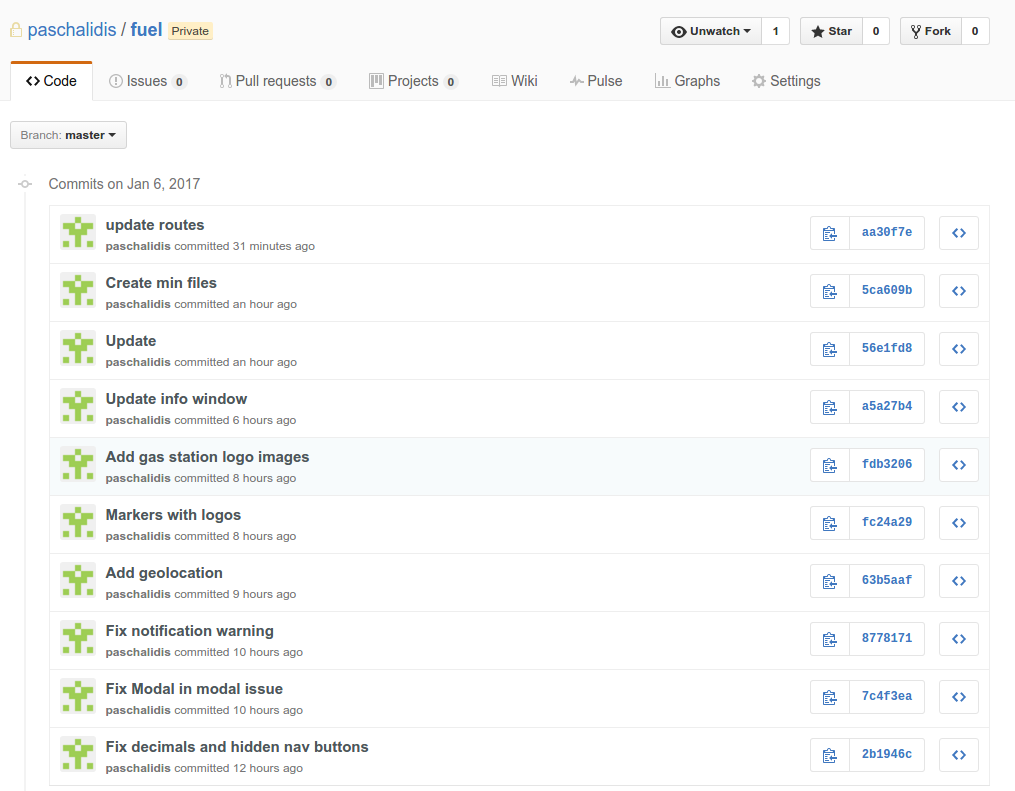
\includegraphics[width=1\textwidth]{img/git.png}
    \label{fig:git}
\end{figure}

\subsection{Βάση Δεδομένων}
Για λόγους ευχρηστίας έγινε πρόσθεση του πεδίου \textbf{id} στους πίνακες \textbf{pricedata} και \textbf{gasstations}, ενώ για τα δικαιώματα των χρηστών (πελάτης, πρατηριούχος) υλοποιήθηκε με το σχεσιακό μοντέλο \textbf{users-and-rights-schema} περισσότερες λεπτομέρειες στο σχεσιακό σχήμα.\ref{fig:db}. Επιπλέον δημιουργήθηκαν τρία views: user-permission, fuel-analytics, pricedata-view.

\begin{figure}[H]
  \caption{Εικόνα από το Σχεσιακό Μοντέλο.}
  \centering
    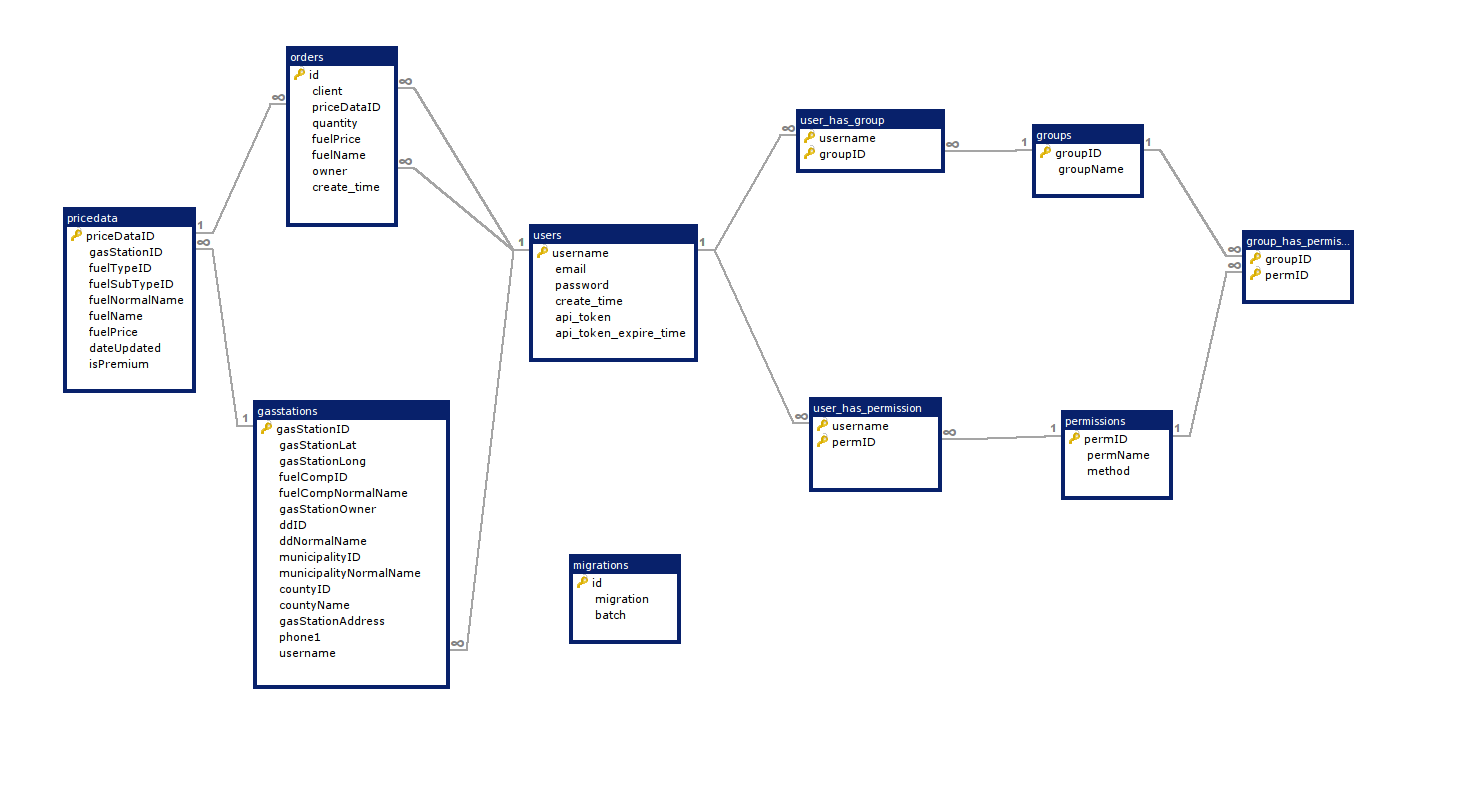
\includegraphics[width=1\textwidth]{img/db-schema.png}
    \label{fig:db}
\end{figure}

\subsection{Καλές Πρακτικές API}
Χρησιμοποιήθηκαν καλές πρακτικές σχεδίασης όπως αυτές παρουσιάστηκαν στις διαλέξεις και για τον έλεγχο και την υλοποίηση των resources η εφαρμογή chrome-postman \cite{chrome-postman}. API URL: \textbf{domain/api/v1/}

\subsubsection{API Resources}
\begin{itemize}
\item GET - gasstations
\item GET - gasstations/count
\item GET - gasstations/id/pricedata
\item GET - pricedata
\item GET - gasstations/analytics
\item POST - login
\item POST - register
\item PUT - pricedata/id
\item POST - orders
\item GET - orders
\end{itemize}

\subsubsection{Fields}
Επιλογή συγκεκριμένων πεδίων με την παράμετρο fields, πχ fields=gasStationID,gasStationLat. \ref{fig:format}

\subsubsection{Where}
Υλοποίηση where statement με το όνομα του πεδίου και την τιμή ή τις τιμές για IN, πχ   gasStationID=1 ή  gasStationID=1,2,3. \ref{fig:format}

\subsubsection{Pagination}
Χρήση pagination με τις εντολές limit και offset και την τιμή του καθενός, πχ limit=10,offset=100. \ref{fig:limit}

\begin{figure}[H]
  \caption{Εικόνα από το API Request Limit και Between.}
  \centering
    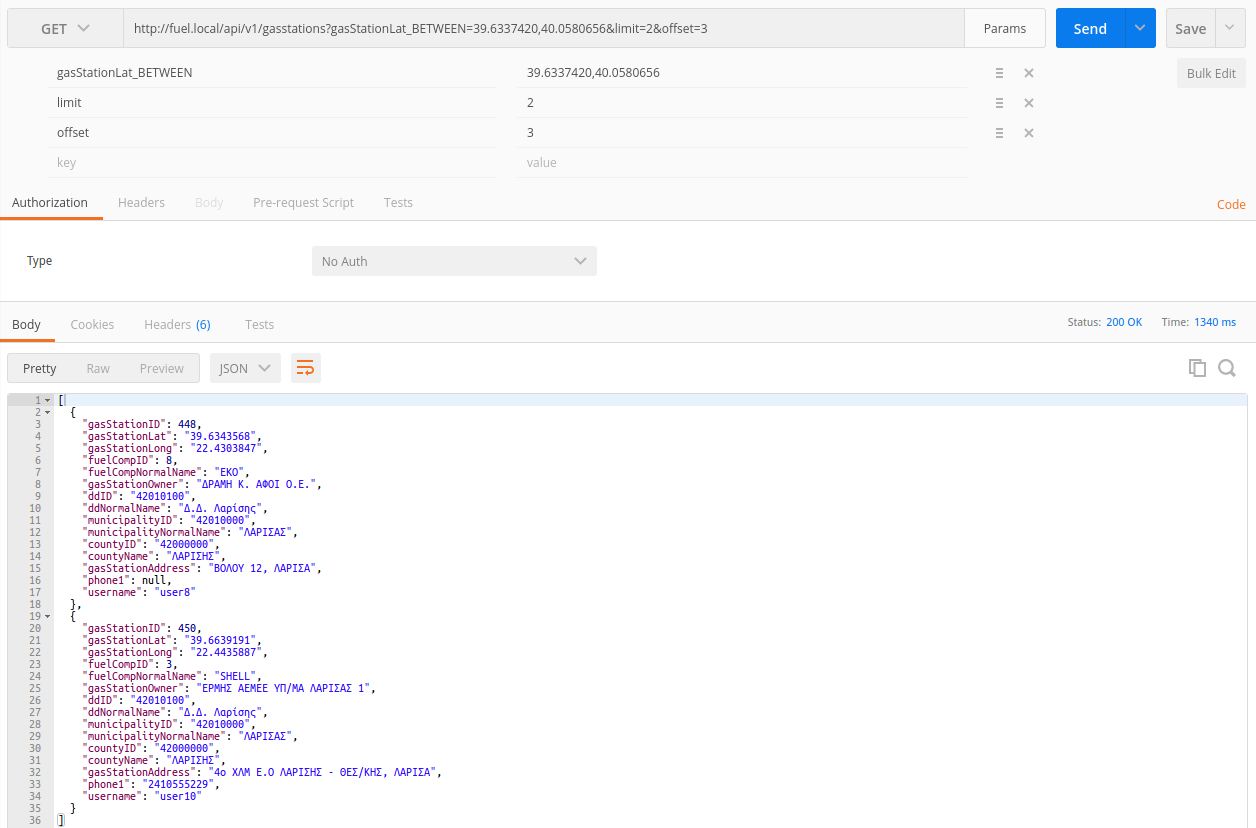
\includegraphics[width=1\textwidth]{img/limit.png}
    \label{fig:limit}
\end{figure}

\subsubsection{Aggregate}
Υλοποίηση συναρτήσεων max, min, avg, count πχ  max=fuelPrice. \ref{fig:aggregate}

\begin{figure}[H]
  \caption{Εικόνα από το API Request με συναρτήσεις και group by.}
  \centering
    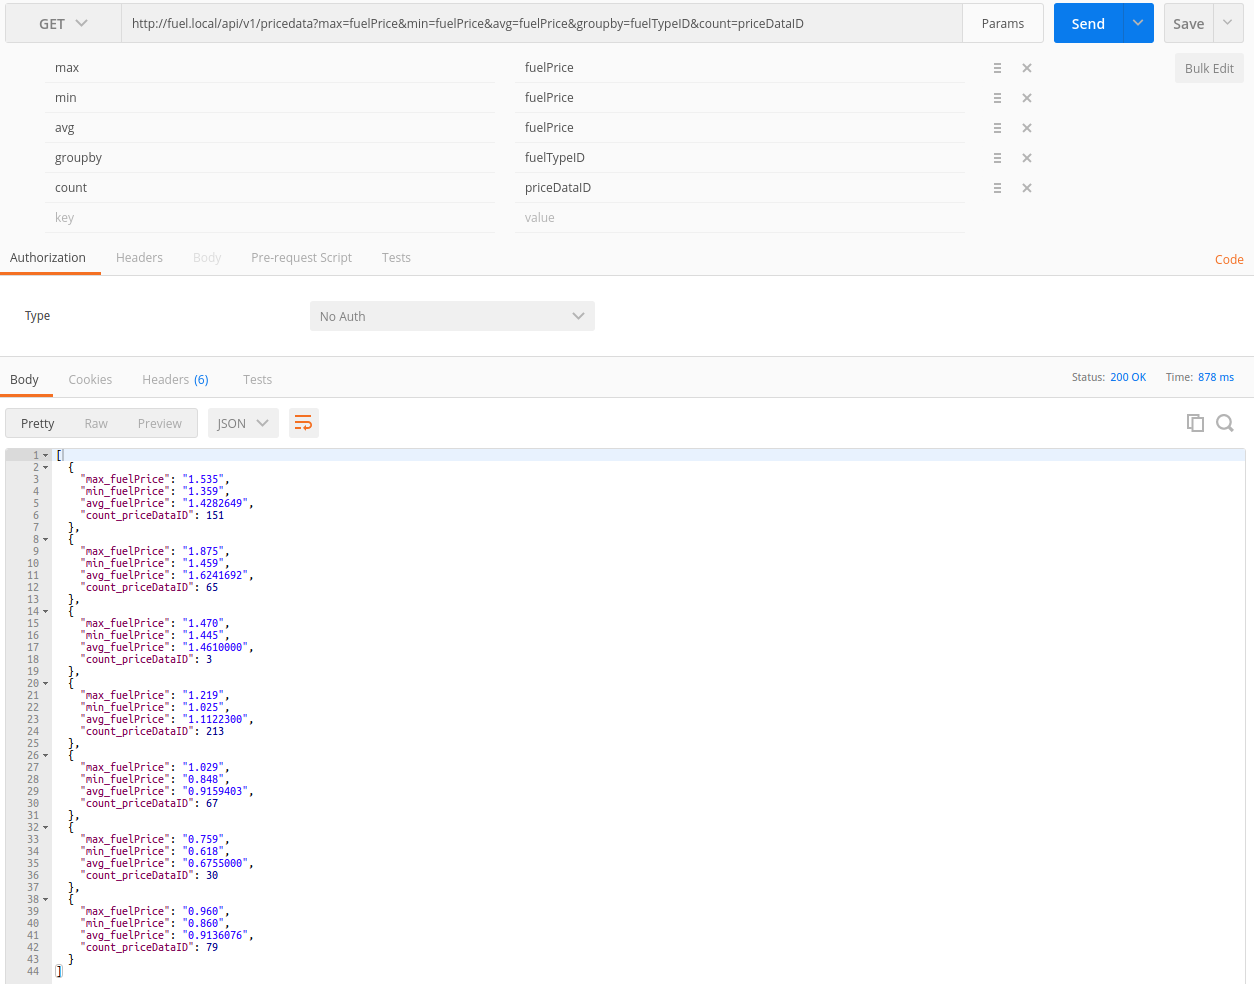
\includegraphics[width=1\textwidth]{img/aggregate.png}
    \label{fig:aggregate}
\end{figure}

\subsubsection{Group By}
Επιλογή για groupby με την παράμετρο groupby, πχ groupby=fuelTypeID. \ref{fig:aggregate}

\subsubsection{Between}
Υλοποίηση του between, πχ gasStationLat\_BETWEEN=39.6337420,40.0580656. \ref{fig:limit}

\subsubsection{Formats}
Επιλογή μορφή δεδομένων με την παράμετρο type=json ή xml. \ref{fig:format}

\begin{figure}[H]
  \caption{Εικόνα από το API Request XML Format.}
  \centering
    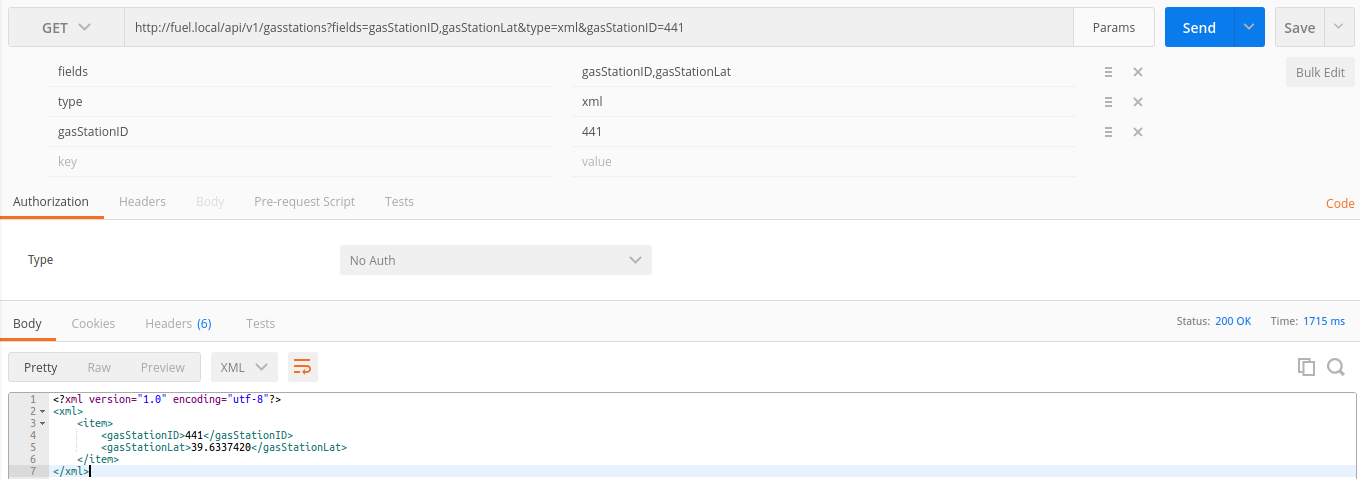
\includegraphics[width=1\textwidth]{img/format.png}
    \label{fig:format}
\end{figure}

\subsubsection{HTTP error}
Με την παράμετρο suppress\_response\_code το API επιστρέφει πάντα http status 200 με μήνυμα λάθους και το response status που θα έπαιρνε. Χωρίς \ref{fig:error} Με \ref{fig:suppress}

\begin{figure}[H]
  \caption{Εικόνα από το API Request με error.}
  \centering
    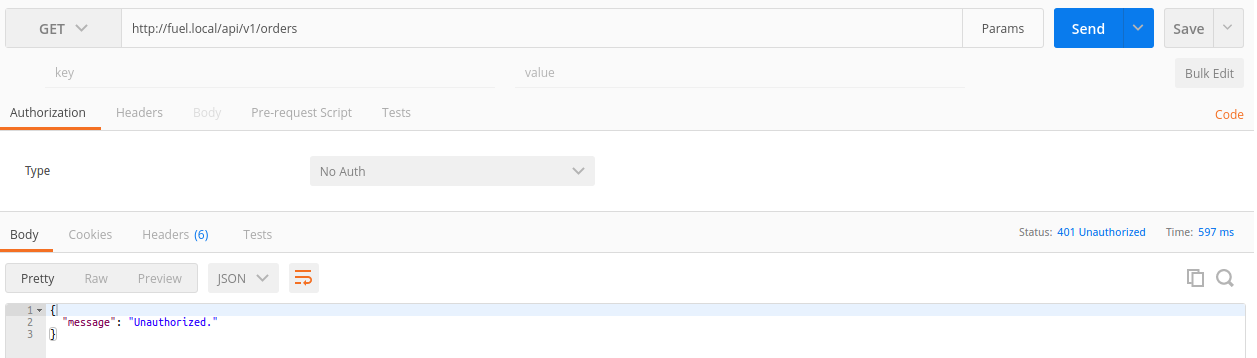
\includegraphics[width=1\textwidth]{img/error.png}
    \label{fig:error}
\end{figure}

\begin{figure}[H]
  \caption{Εικόνα από το API Request με error και suppress response.}
  \centering
    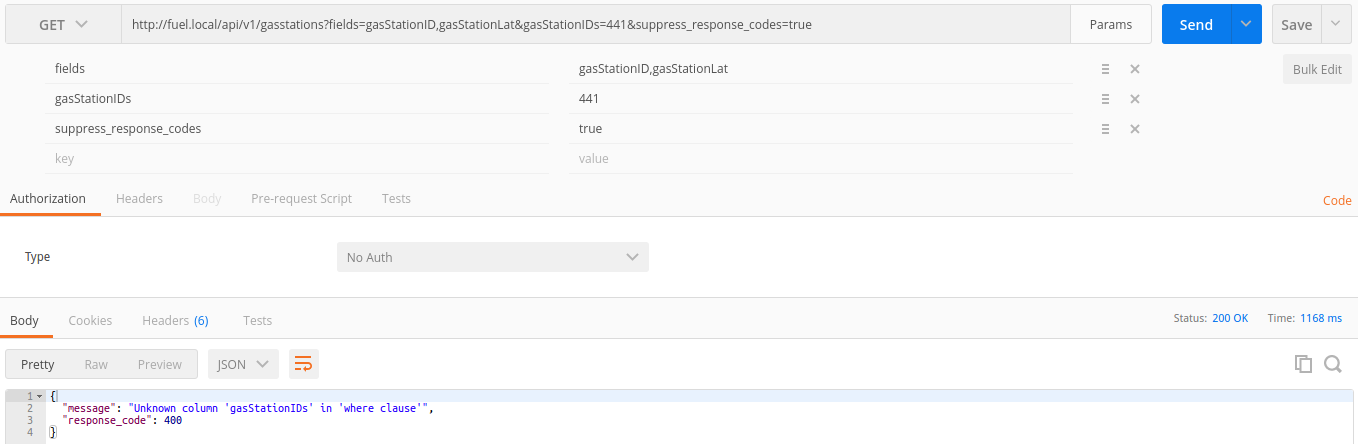
\includegraphics[width=1\textwidth]{img/suppress.png}
    \label{fig:suppress}
\end{figure}

\subsection{Πλαίσιο Λογισμικού - CSS,JS}
Για την υλοποίηση της εφαρμογής Single Page RIA χρησιμοποιήθηκε το framework \textbf{Βootsrap} \cite{bootstrap}
το οποίο παρέχει πολλές λειτουργίες σε HTML, CSS και JS. Για τις ajax κλήσης χρησιμοποιήθηκε η βιβλιοθήκη \textbf{jQuery} \cite{jquery} που είναι εύχρηστη και για τα μηνύματα προς τον χρήστη το plugin \textbf{Notify.js} \cite{notify}.

\subsection{Τεχνικές Βελτιστοποίησης}
Για την βελτιστοποιήσει της εφαρμογής χρησιμοποιήθηκαν τεχνικές όπως αυτές παρουσιάστηκαν στις διαλέξεις. Τα αρχεία \textbf{CSS} ενσωματώθηκαν στο head ενώ τα \textbf{JS} στο τέλος της σελίδας έτσι ώστε ο browser να δημιουργήσει πιο γρήγορα τη σελίδα. Έγινε αποφύγει των \textbf{redirects} σε όλες τις κλήσης προς τον srever με χρήση μιας \textbf{πλάγιας καθέτου} στο τέλος του url και με την χρήση της παραμέτρου \textbf{fields} επιλέχθηκαν μόνο τα απαραίτητα πεδία για να μειωθεί ο όγκος τον δεδομένων. Τέλος για την συμπίεση των αρχείων css και js χρησιμοποιήθηκε το εργαλείο \textbf{cssminifier} \cite{cssminifier}.

\subsection{Google APIs}
Η εφαρμογή δείχνει σε χάρτη τα πρατήρια της περιοχής ενδιαφέροντος με του \textbf{Google Maps APIs} \cite{google-map}.και για την εποπτική προβολή της αγοράς δημιουργήθηκαν δύο γραφήματα αξιοποιώντας τα \textbf{Google Charts} \cite{google-chart}.